\documentclass{article}
\usepackage[utf8]{inputenc}
\usepackage[english]{babel}
\usepackage[font=small,labelfont=bf]{caption}
\usepackage{geometry}
\usepackage{natbib}
\usepackage{pxfonts}
\usepackage{graphicx}
\usepackage{newfloat}
\usepackage{setspace}
%\doublespacing


\title{\textit{Supplemental materials for}: How is experience transformed into memory?}
\author{Andrew C. Heusser, Paxton C. Fitzpatrick, and Jeremy R. Manning\\Department of Psychological and Brain Sciences\\Dartmouth College, Hanover, NH 03755, USA\\Corresponding author: jeremy.r.manning@dartmouth.edu}

\bibliographystyle{apa}

\begin{document}
\maketitle

\setcounter{equation}{0}
\setcounter{figure}{0}
\setcounter{table}{0}
\setcounter{page}{1}
\setcounter{section}{0}
\makeatletter
\renewcommand{\theequation}{S\arabic{equation}}
\renewcommand{\thefigure}{S\arabic{figure}}
\renewcommand{\bibnumfmt}[1]{[S#1]}
\renewcommand{\citenumfont}[1]{S#1}


\section*{Overview}
This document provides additional details about the methods we used in the main text.  We also include some additional figures referenced in the main text.

\section*{Additional details about topic modeling methods and results}
\subsection*{Optimizing topic model parameters}
In order to create accurate video and recall models, we used an optimization method that was driven by our ability to explain hand-annotated memory performance metrics collected by \cite{ChenEtal17}.  Specifically, we \textbf{JRM STOPPED HERE}
% argmax \omega (movie window size), \rho (recall window size), and K (number of topics)

\begin{figure}[tp]
\centering
\includegraphics[width=1\textwidth]{figs/parameter_search}
\caption{\small \textbf{Optimizing video model parameters.} Matrices representing the correlation value between hand-annotated memory performance and mean squared error between video model and recall model. Best fitting model was 100 topics, 50 video window size and 10 recall window size}
\label{fig:paramsearch}
\end{figure}

The optimized model converged on 28 unique topics that were assigned non-zero weights over the course of the video.  We provide a list of the top ten highest-weighted words from each topic in Figure~\ref{fig:topics}.





\begin{figure}[tp]
\centering
\includegraphics[width=0.75\textwidth]{figs/topic_words}
\caption{\small \textbf{Topics discovered in \textit{Sherlock}.} We applied a topic model to hand-annotated information about 1000 scenes spanning the 45 minute episode.  We identified 28 unique topics with non-zero weights (we used $K=100$ topics to fit the model).  Each topic comprises a distribution of weights over all words in the vocabulary.  For each topic, we show the words with the 10 largest weights, along with a suggested description of the topic.}
\label{fig:topics}
\end{figure}


\subsection*{Feature importance}
To determine the contribution of each feature to the structure of the video topic proportions, we conducted a ``leave one out'' anlaysis.  Specifically, we compared the original video topic trajectory (created using all hand-annotated features from the 1000 hand-annotated scenes spanning the \textit{Sherlock episode}; see \textit{Methods} for a full list of features) with video trajectories created using all but one type of feature.  We created temporal correlation matrices for each trajectory (using the topic proportions matrices) and correlated the upper triangles of each impoverished trajectory with the original feature-complete trajectory.  Observing a lower correlation between an impoverished trajectory (holding out a particular feature) and the feature-complete trajectory would suggest that the given feature played a more prominent role in shaping the structue of the feature-complete trajectory.  We found that hand-annotated narrative details provided the most structure to the feature-complete trajectory, whereas transcriptions of onscreen text provided the least structure (Fig.~\ref{fig:feature-importance}A).

\begin{figure}[tb]
\centering
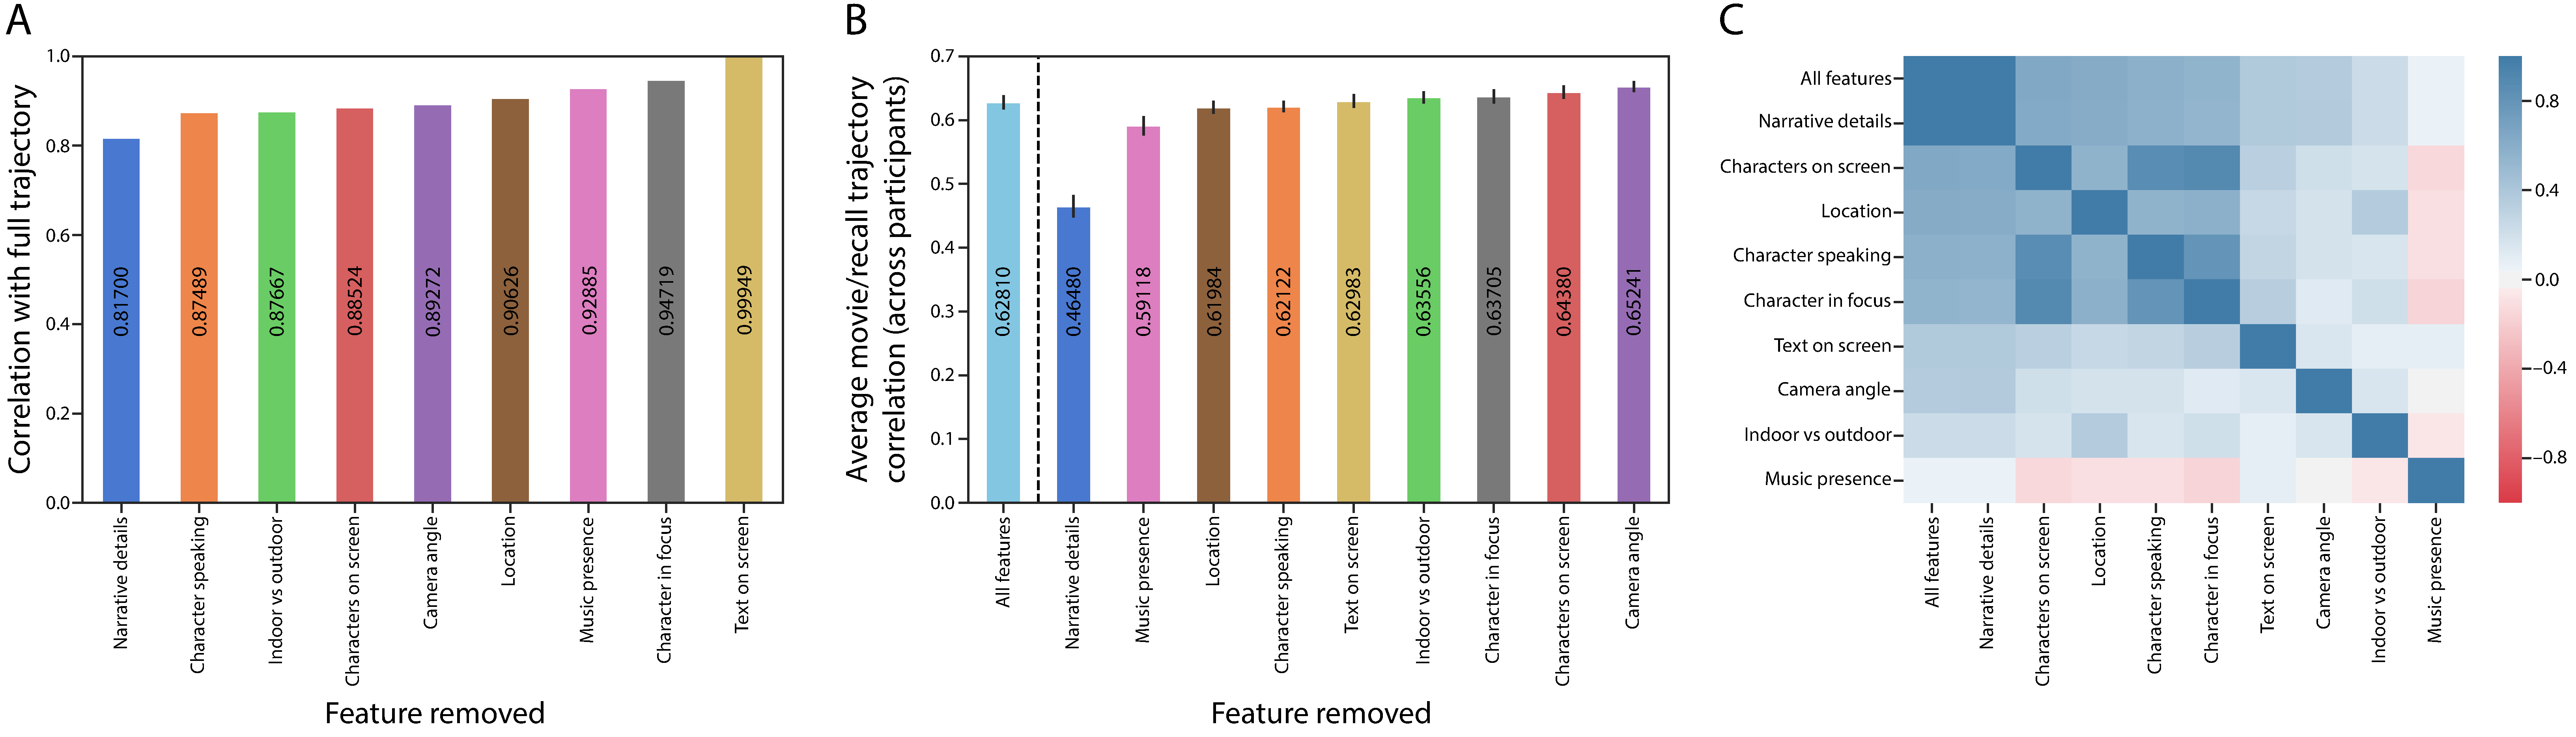
\includegraphics[width=1\textwidth]{figs/feature_value}
\caption{\small \textbf{Impact of individual features on topic modeling analysis.} \textbf{A.} Contribution of each feature to model structure. Bars represent the correlation of a video model trained in the absence of a given feature to the model trained on all features. \textbf{B.} Contribution of each feature to video model/recall model relationship. The leftmost bar represents the across-participants mean correlation between the video model and recall models trained on all features. Subsequent bars represent the same relationship between video and recall models trained in the absence of a given feature. Error bars are the standard error of the mean across participants. \textbf{C.}  Individual feature trajectory similarity matrix. The first row/column is the topic trajectory the full video model. Each subsequent row/column is that of a single feature. Shading corresponds to the value of the correlation coefficient (Pearson's $r$) .}
\label{fig:feature-importance}
\end{figure}

We also carried out an analysis of which annotated features tended to shape aspects of the video topic trajectory that were preserved in participants' recalls.  Specifically, we computed the timepoint-by-timepoint correlation matrix of the video topic trajectory, and correlated its upper triangle with the timepoint-by-timepoint correlation matrices of each participant's recall topic trajectory (resampled using linear interpolation to have the same number of timepoints as the video trajectory).  This yielded a single correlation coefficient for each participant.  We then carried out a series of analyses whereby we repeated the analysis with each annotated feature held out in turn.  Observing a lower correlation between the video and recall trajectories (when a given feature was held out) would indicate that the feature tends to be preserved in participants' recalls.  We found that hand-annotated narrative details were the most preserved type of feature, whereas information about the camera angle tended not to feature in participants' recalls (Fig.~\ref{fig:feature-importance}B).

Next, we wondered how the different types of features might relate.  For example, knowing which characters are on screen during a given scene may also provide information about which characters are speaking.  We computed video topic trajectories for each feature in turn, and then compared the temporal correlation matrices of all pairs of features.  This provided additional confirmation that the full model (including all types of features) was largely driven by narrative details.  We also found that character-driven features (characters on screen, characters speaking, and characters in focus) were strongly correlated.  Other details, such as the presense or absense of music, led to very different topic trajectories (Fig.~\ref{fig:feature-importance}C).




\section*{Additional analyses of memory performance}

\section*{Naturalistic extensions of classic list-learning analyses}
Just like in a traditional free recall list-learning experiment where participants view a list of words and then verbally recall them, our video-recall matching analysis approach affords us the ability to analyze memory in the same way. The recalled events can be treated as ``items'' analogous to words recalled in a list-learning study. Here, we sought to characterize memory performance/dynamics by extending classic analyses originally designed for list-learning experiments to more naturalistic settings.

First, we asked whether the estimated number of recall events ($k$) by participant was related to hand-annotated accuracy as published in Chen et al. (2017).  We found a strong positive correlation where participants with a greater number of recall events also had better overall memory performance (Pearson's $r(16) = 0.67, p = 0.003$). Then, we considered how participants initiated the recall sequence (known in the literature as the `probability of first recall' or `PFR'). We found that participants tended to initiate their recall sequences with the first few events (Supp. Fig.~\ref{fig:list-learning}A), which is qualitatively very similar to previously published list learning experiments ~\citep{HowaKaha99}. Next, we considered another well-studied memory measure in the list-learning literature, the lag conditional response probability curve (or lag-CRP) ~\citep{Kaha96}. The result suggests a strong bias to transition sequentially events in the forward direction (Supp. Fig.~\ref{fig:list-learning}B). Finally, we assessed memory performance for each event in the video as a function of its serial position during encoding (Supp. Fig.~\ref{fig:list-learning}C). We did not observe the classic ``primacy'' and ``recency'' pattern which is prevalent in the literature ~\citep{Murd62a}. We also considered two additional across-participant measures of recall that characterize memory organization: temporal clustering and semantic clustering. We found that participants who clustered in time also recalled a greater number of events (Pearson's $r(16) = 0.62, p = 0.007$). Next, we assessed semantic clustering. We found that the semantic clustering score was related to memory performance across participants (Pearson's $r(16) = 0.55, p = 0.02$).  Thus, participants who organized their recalls with respect to the semantic information contained in the scene had better memory performance.

\section*{Additional measures of naturalistic memory}
To quantify the similarity between the video model and individual recall models, we considered a number of novel metrics.  First, we tested whether each participant's recall model matched the video model in a general sense. To do this, for each participant we filtered the video model to only include the events that the participant remembered and computed the root mean squared difference (RMSD) between the video model and the recall model. As an example, if the participant remembered all the events in order (with perfect precision), the expected distance value would be 0. However, if they remembered a subset of events, events out of order, or with low precision, the expected distance would be greater than 0. To assess significance, we performed a permutation test where we circularly shifted the recall model (10000 times) and recomputed the RMSD. The recall model significantly matched the video model for nine of the participants ($p < 0.05$, participants: 3-4, 8-13, 17 and the p-value for the rest of the participants was less than .25). Furthermore, the RMSD values were significantly correlated to hand annotated memory performance across participants (Pearson's $r(16) =-.57, p = 0.016$). Thus, a closer match between the video and recall event models was related to better recall performance.

Next, we tested whether participants who recalled more events were also more precise in their recollections. For each participant, we computed the correlation between each recall event and its matching video event (only for the events which they recalled). This resulted in a single number for each recalled event indexing how similar the recall event was to its matching video event (i.e the ``precision'' of the recall). We then averaged the correlations within participant. In line with our prediction, there was a strong correlation between hand annotated memory performance and precision suggesting that participants who remembered more events also remembered them more veridically (Pearson's $r(16) = 0.74, p = 0.0006$).

Then, we considered the distinctiveness of each recall event. That is, how uniquely a recall event matched a given video event compared to all other video events. We hypothesized that participants with high memory performance might describe each event in a more distinctive way (relative to those with lower memory performance who might describe events in a more general way). To this end, we computed a `distinctiveness' score for each participant (i.e., 1 - the correlation between a recall event and all non-matching video events).  Then, we averaged this measure over recall events within participant.  We found that participants with higher hand annotated memory performance also had higher distinctiveness scores (Pearson's $r(16) = 0.8, p = 0.0001$).

Lastly, we tested whether participants with better memory performance were also more likely to remember the events in order.  For each participant, we computed the Spearman rank correlation between the order of events that the participant recalled and the actual order of events (filtering events that were actually recalled).  We found that participants who recalled more events also recalled more of them in order (Pearson's $r(16) = 0.5, p = 0.04$). In summary, we found that better memory performance was associated with more precise, distinctive and ordered recalls.


\subsection*{List-learning analyses}
\textbf{Overall Accuracy.}  To get an overall measure of the quantity of information recalled, we computed the proportion of sucessfully recalled events by counting the number of unique recall events identified by the HMM model and dividing by the total number of video events.  We performed this analysis for each participant separately.

\textbf{Probability of first recall (PFR).}  The (PFR) analysis represents the probability that an item will be recalled first as a function of its serial position during encoding. We initialized a \# of participants (17) by \# of video events (34) matrix. Then for each participant, we found the index of the video event that was recalled first and filled in that index in the matrix with a 1.  Finally, we averaged over the rows of the matrix, resulting in a 1 by 34 array representing the proportion of participant that recalled an event as a function of serial position during encoding.

\textbf{Lag conditional probability curve (lag-CRP).} The lag-CRP represents the probability that the next item recalled will be of lag $i$ from the just recalled item. For each recall transition, we computed the lag between the current recall event and the next recall event, normalizing by the total number of possible transitions.  This resulted in a \# of participants (17) by lags (-33:+33) matrix. We averaged over the rows of this matrix to get a group-averaged lag-CRP.

\textbf{Serial position curve (SPC).} The SPC represents the proportion of participants that remember an item as a function of its serial position during encoding. We initialized a \# of participants (17) by \# of video events (34) matrix. Then, for each recall event (and each participant), we found the index of the video event that was recalled and filled it in with a 1. This resulted in a matrix where 1s indicate the successful recall of an event in serial position $n$ and zeros indicate the lack of recall for that event.  Lastly, we averaged over the rows of the matrix to get a 1 by 34 array representing the proportion of participants that recalled an event as a function of its serial position.

\textbf{Temporal clustering.} Temporal clustering measures the extent to which participants group their recall responses according to encoding position ~\citep{PolyEtal09}. For instance, if the participant recalled each item in the presentation order, this would result in a score of 1. If the participant recalled randomly with respect to presentation order, this would result in a score of ~.5.  For each event transition (and separately for each participant), we computed the rank similarity (euclidean distance) between the presentation position  of the current and next recall events. The scores were then averaged within participant to get a single number representing the extent of temporal clustering exhibited by a given participant.

\textbf{Semantic clustering.} Similar to temporal clustering, semantic clustering measures the extent to which participants group their recall responses according to semantic similarity ~\citep{PolyEtal09}. Here, we are using the topic vectors for each event as a proxy for its semantic content. Thus, similarity between the semantic content for two events can be computed by correlating their respective topic vectors.  For instance, if each consecutive recall was the next most similar event (in terms of its s), this would result in a score of ~1. If the participant recalled randomly with respect to semantic similarity, this would result in a score of ~.5.  For each event transition (and separately for each participant), we computed the rank similarity (correlation distance) between the current recall event and the next recall event. The scores were then averaged within participant to get a single number representing the extent of semantic clustering exhibited by a given participant.

\subsection*{Additional measures of naturalistic memory}
\textbf{Precision.} This measure gives us an indication of the specific match between a video event and recall event, where values approaching 1 are highly precise and lower values are inprecise.  We defined ``precision'' as the correlation between a recall event and its matching (i.e., argmax) video event.

\textbf{Distinctiveness.} Distinctiveness quantifies how similar a recall event is to all non-matching video events.  It provides a metric of how uniquely a particular recall event describes a particular video event.  To compute it, a given recall event is correlated to all video events, the argmax is removed and the rest of the values are averaged. The resulting value is subtracted from 1 such that larger values indicate a more distinctive recall event.

\begin{figure}[tb]
\centering
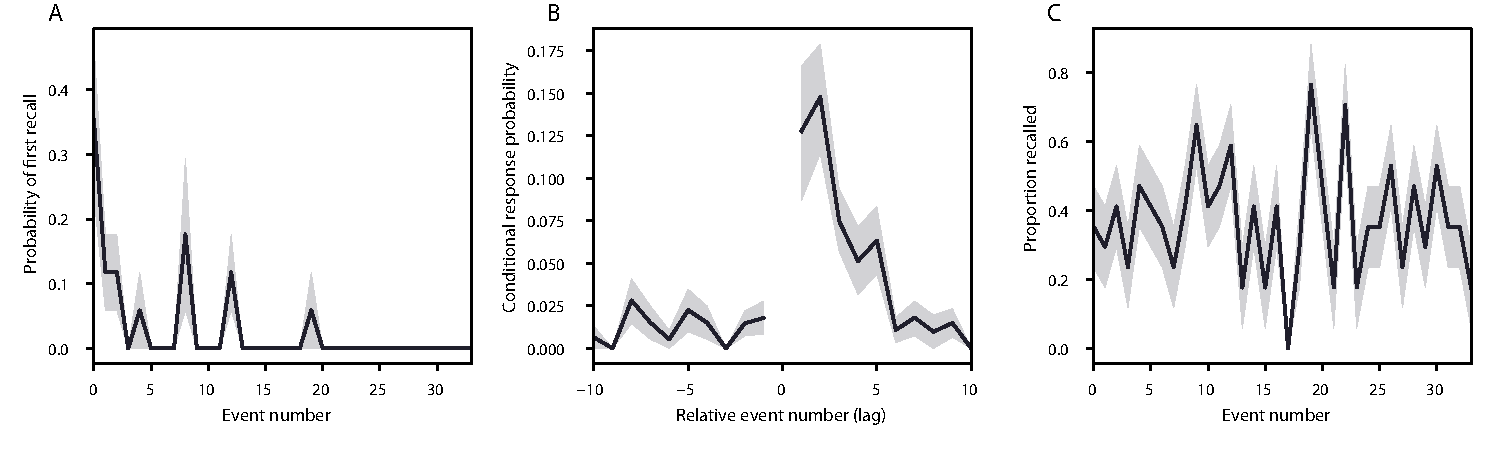
\includegraphics[width=1\textwidth]{figs/list_learning}
\caption{\small \textbf{Naturalistic extensions of classic list-learning memory analyses.} A). The probability of first recall as a function of the serial position of the event during encoding. B). A lag-conditional response probability curve. Given recall of event i, the probability that the next recalled item will be from serial position i +/- lag. C). Proportion of events recalled as a function of serial position. All error bars are the standard error of the mean derived from a bootstrap resampling procedure.}
\label{fig:list-learning}
\end{figure}

\section*{Participant-level results referenced in the main text}

% Supplemental materials


\begin{figure}[tp]
\centering
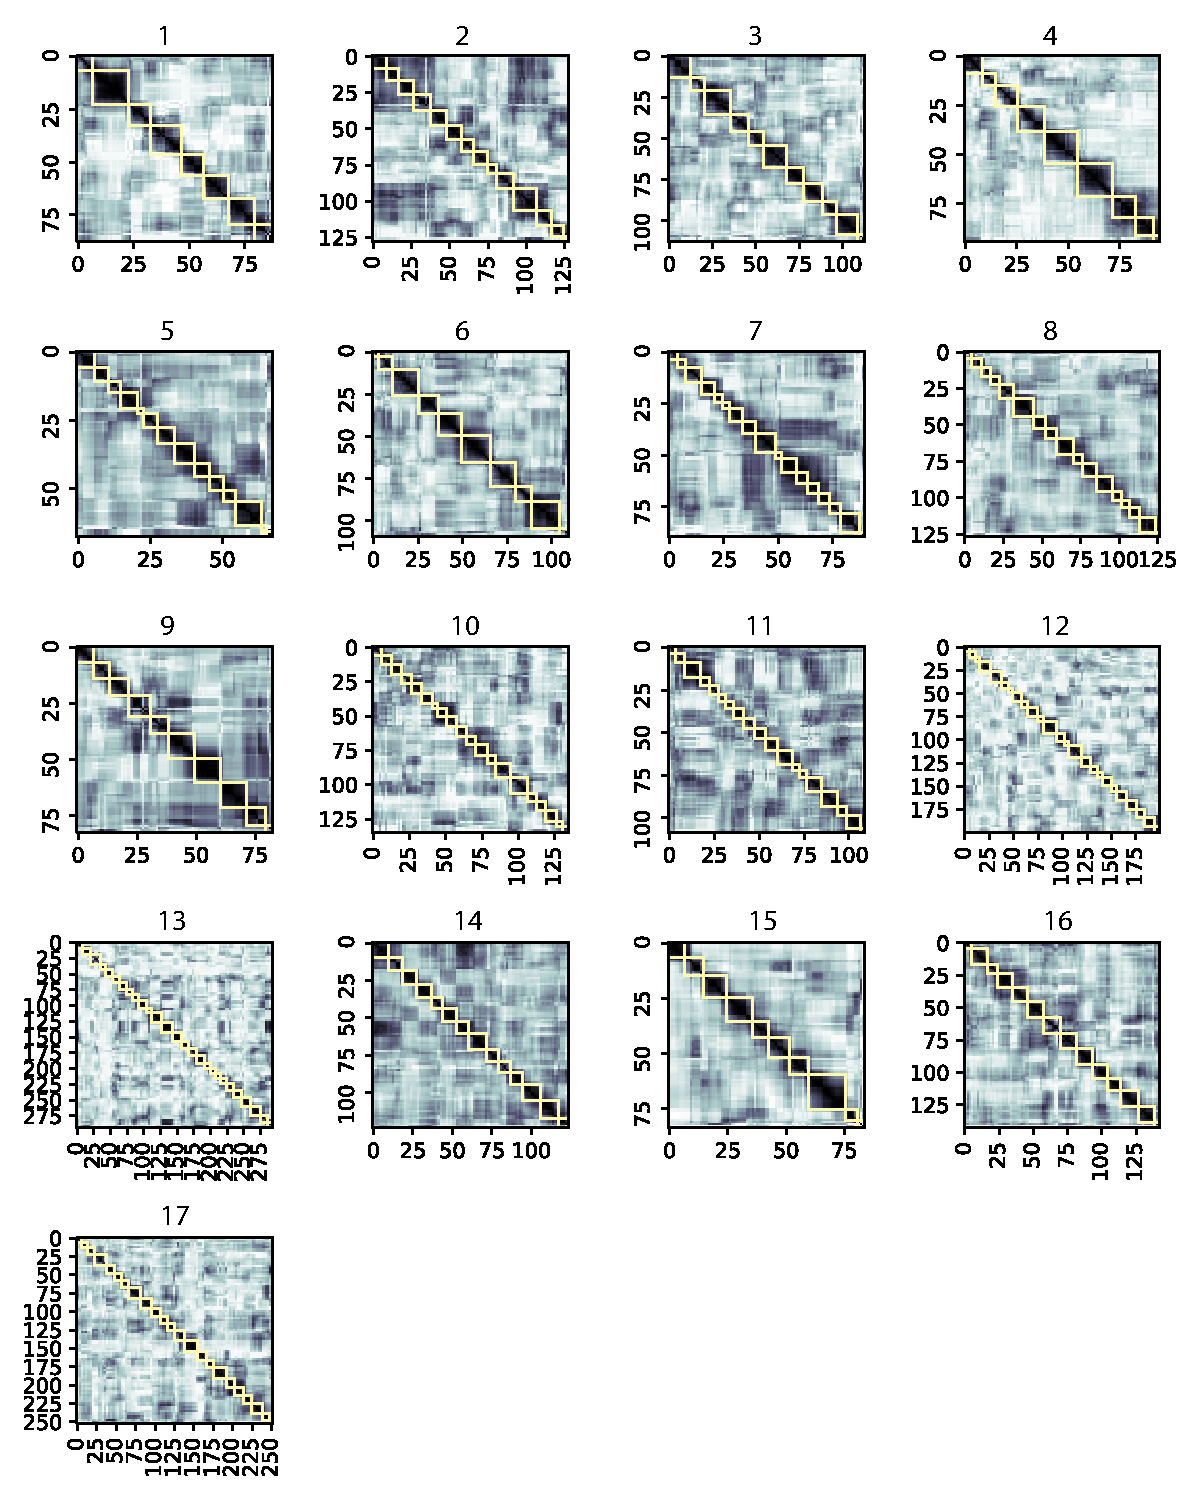
\includegraphics[width=1\textwidth]{figs/corrmats}
\caption{\small \textbf{Recall model correlation matrices and event segmentation fits.} Each participant's timepoint-by-timepoint recall correlation matrix.  The yellow boxes represent ``events'' identified by a hidden Markov model.}
\label{fig:corrmats}
\end{figure}

\begin{figure}[tp]
\centering
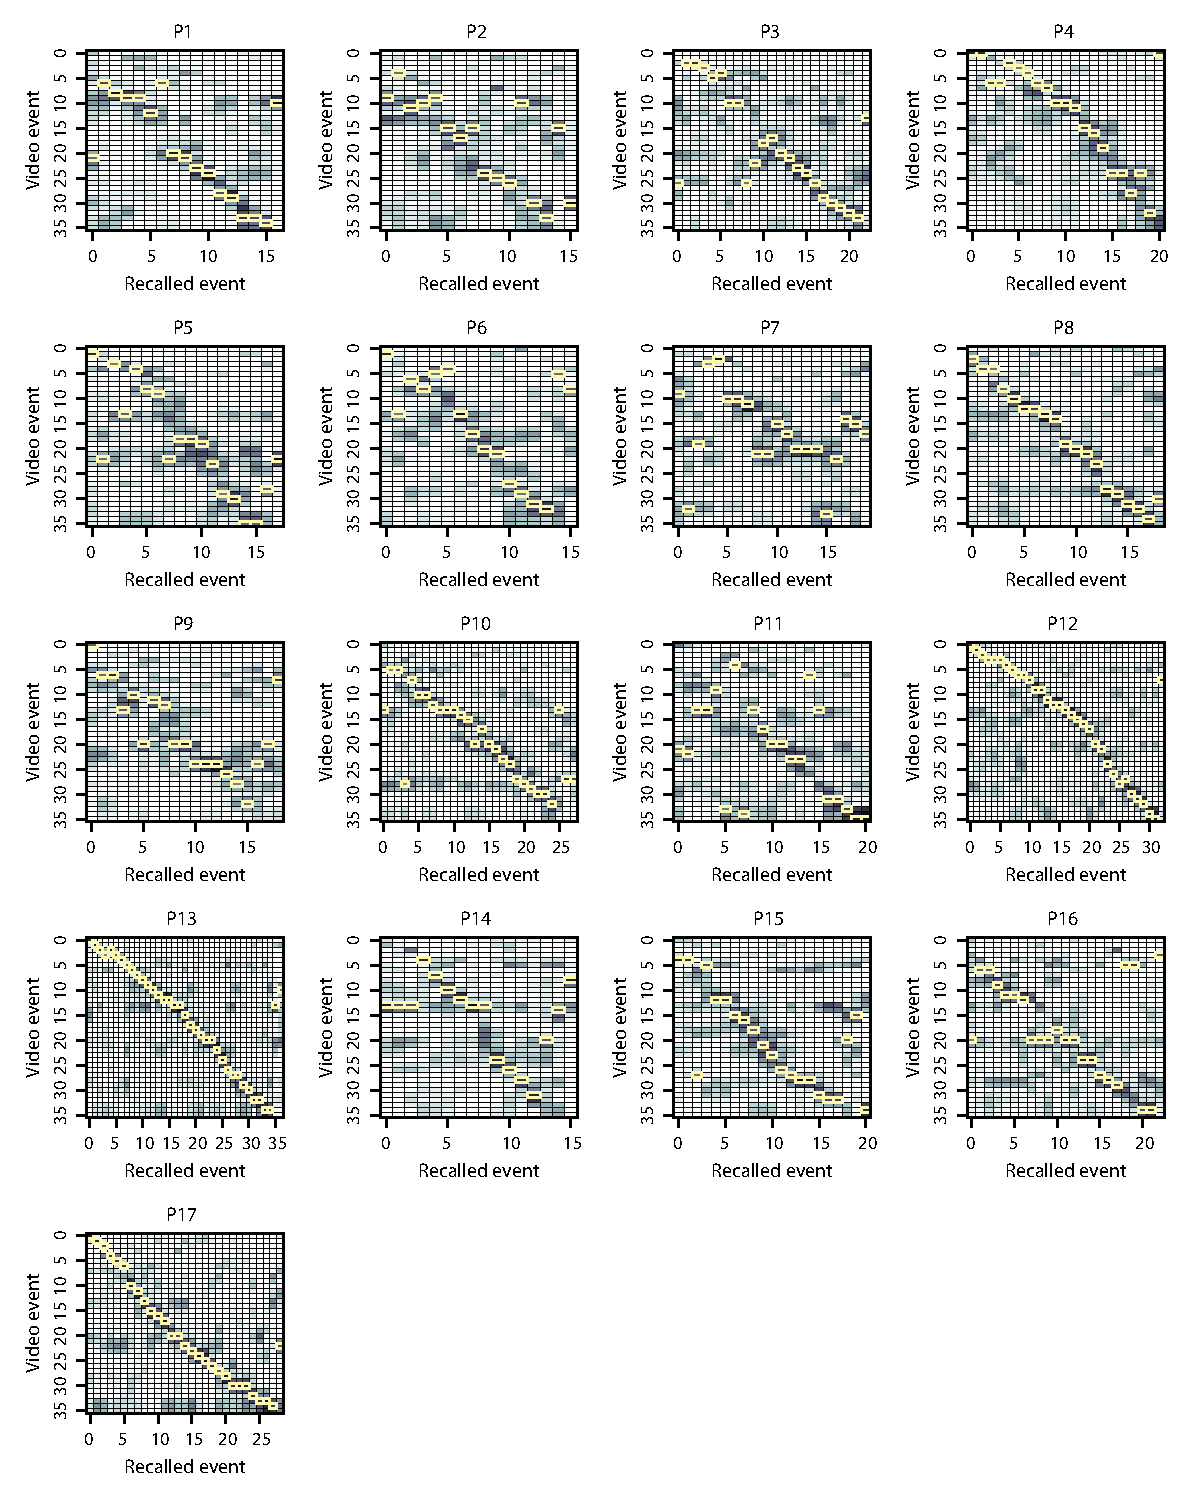
\includegraphics[width=1\textwidth]{figs/matchmats}
\caption{\small \textbf{Video-recall event model correlation matrices.} Each participant's video event by recall event correlation matrix.  The yellow boxes represent the maximum correlation in each column.}
\label{fig:matchmats}
\end{figure}









%\newpage
\renewcommand{\refname}{Supplemental references}
\bibliography{memlab}


\end{document}
